\documentclass{template}

\addbibresource{Bibliographie.bib} % ajout bibliographie

\begin{document}
% Définition des informations pour la page de garde
\newcommand{\supervisor}{Gravier Laurent, Khaoula Hanin}

% Page de garde
\begin{titlepage}
    \begin{center}
        
\includegraphics[width=0.3\textwidth]{png/HEIG_1.png} % Logo de votre université
        \vspace{8cm}
        
        {\Large HEIG-VD}
        
        \vspace{1cm}
        \textbf{\Huge Rapport de Physique}
        \textbf{\Huge \\sur}
        \vspace{0.5cm}
        \textbf{\Huge \\Les Ondes Accoustiques (Solides)}

        \vspace{1.5cm}
        \large{Réalisé par}
        
        \vspace{0.3cm}
        {\Large \textbf{Pitteloud Célien, Rivera Evan, Roeslin Olivier}}
        
        \vspace{0.5 cm}
        \large{Sous la supervision de}
        
        \vspace{0.3cm}
        {\Large \textbf{\supervisor}}
        
        \vfill
        %
\includegraphics[width=1\textwidth]{HEIG-VD_logo.png} % Logo du département de physique
        
        \vfill
        \large{\today}
        
    \end{center}
\end{titlepage}


\tableofcontents % Table des matières
\newpage
\listoffigures % Table des figures
\newpage
\listoftables % Liste des tables
\newpage
\section{Introduction}
\subsection{Contexte}

\subsubsection{\large Le cadre}
~\cite{Polycop-Ondes}

\subsubsection{\large Etat de l'art (SOTA)}
~\cite{wikipedia-onde}


\subsubsection{\large Domaines d'applications}

\subsection{Objectifs}

\subsubsection{\large Objectifs spécifiques et listes de tâches}
\newpage
\section{Manipulation 1 "Mesurer la vitesse de propagation du son dans des
barreaux solides par méthode de résonance en mode continu."}
\subsection{\large Approches / Méthodes}
\subsubsection{\large Rappels Théoriques}

\paragraph{Introduction}

\begin{figure}[h]
    \centering
    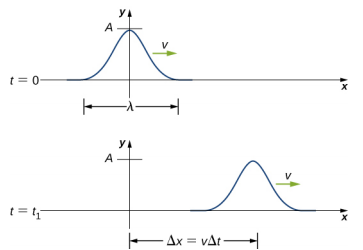
\includegraphics[width=10cm]{png/onde.png}
    \caption{Onde progressive à une dimension.~\cite{image-onde-progressive}}
\end{figure}

\paragraph{Equations physiques}
ok
c'est cool
salut
hello
\begin{figure}[h]
    \centering
    \begin{minipage}{0.45\textwidth}
        \centering
        \adjustbox{max width=\linewidth}{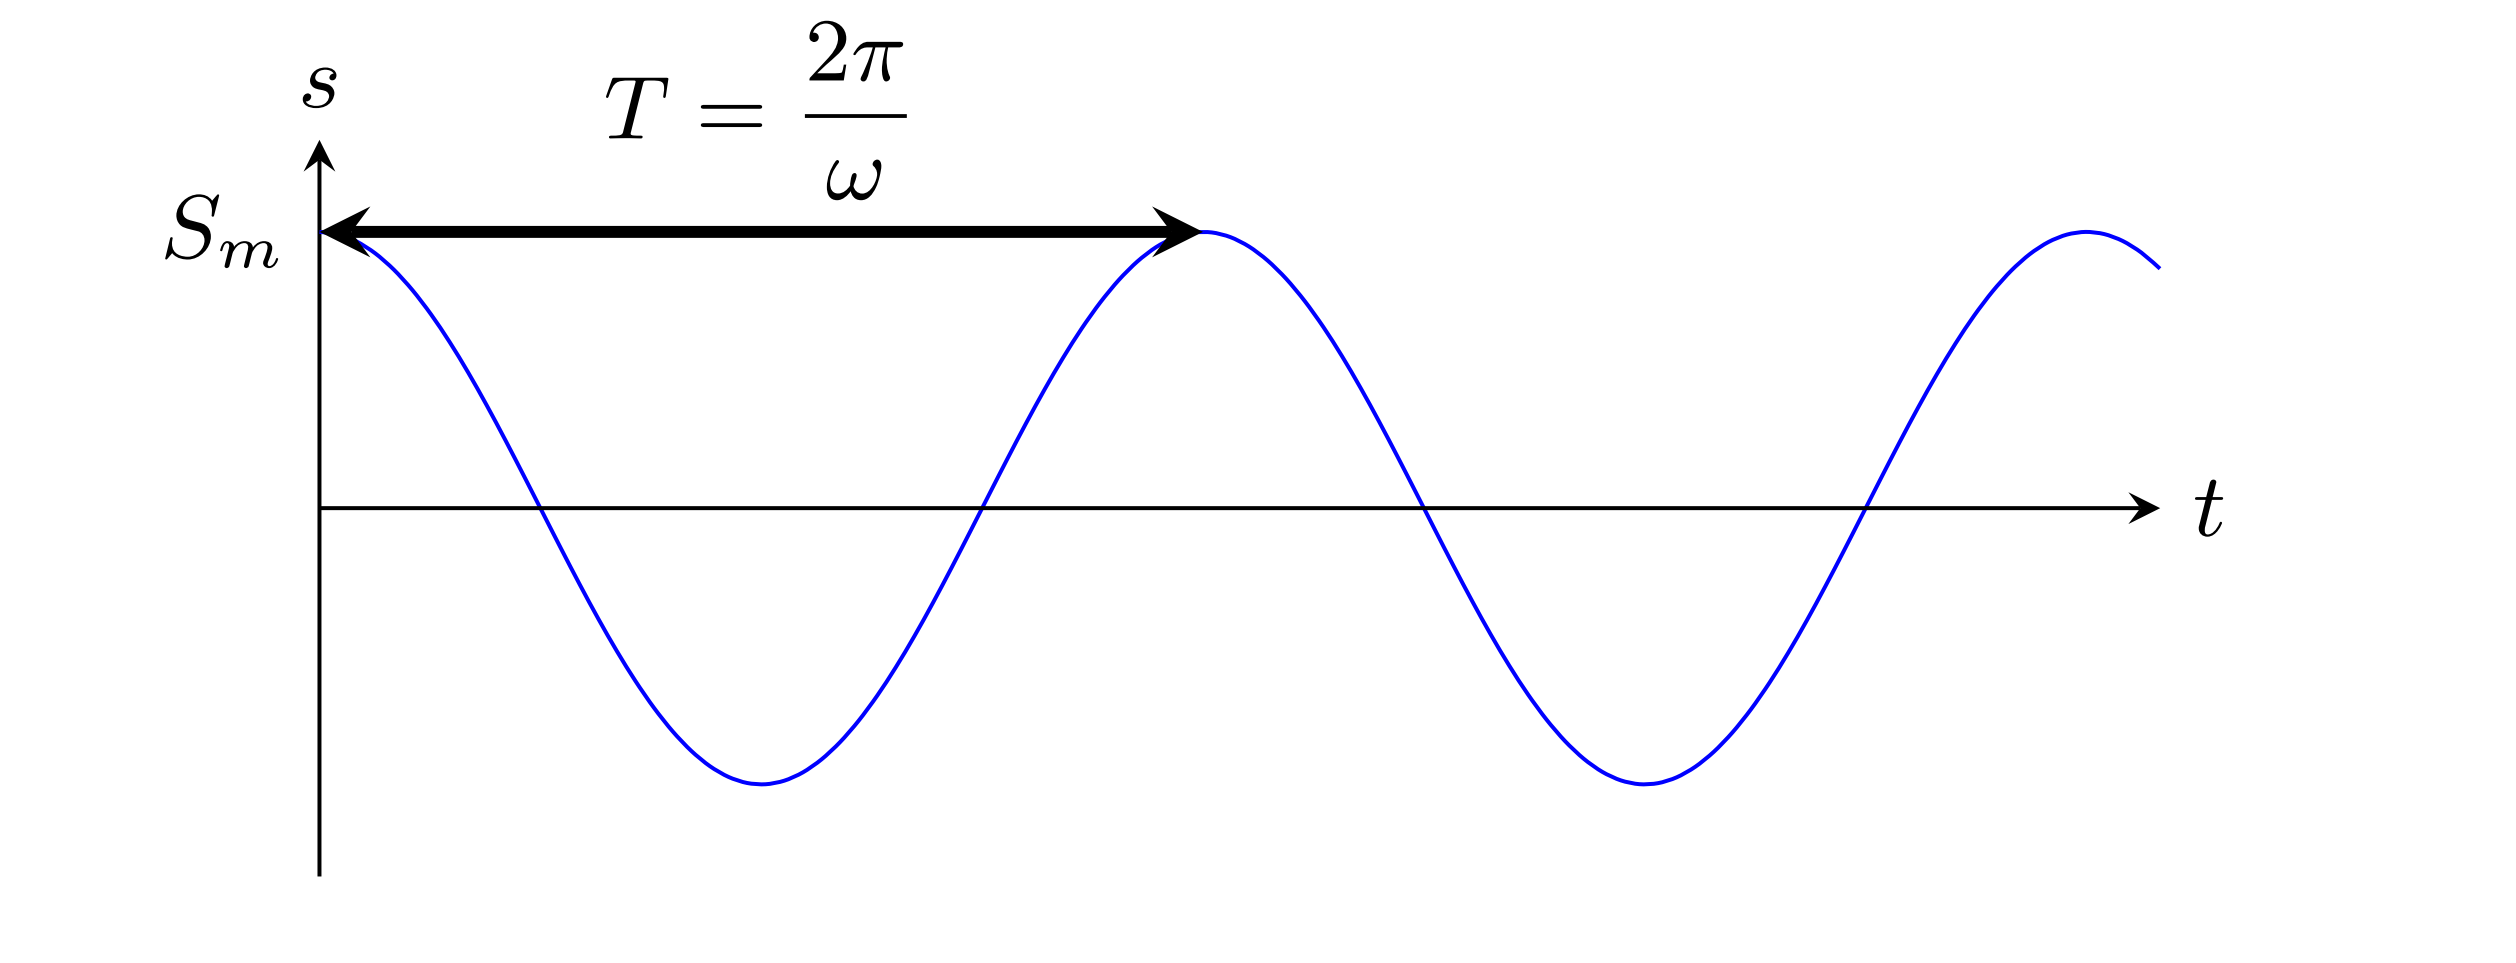
\includegraphics{png/evolution_temporelle.png}}
        \caption{Evolution temporelle d'un point donné du milieu.~\cite{propagation-onde}}
    \end{minipage}
    \hfill
    \begin{minipage}{0.45\textwidth}
        \centering
        \adjustbox{max width=\linewidth}{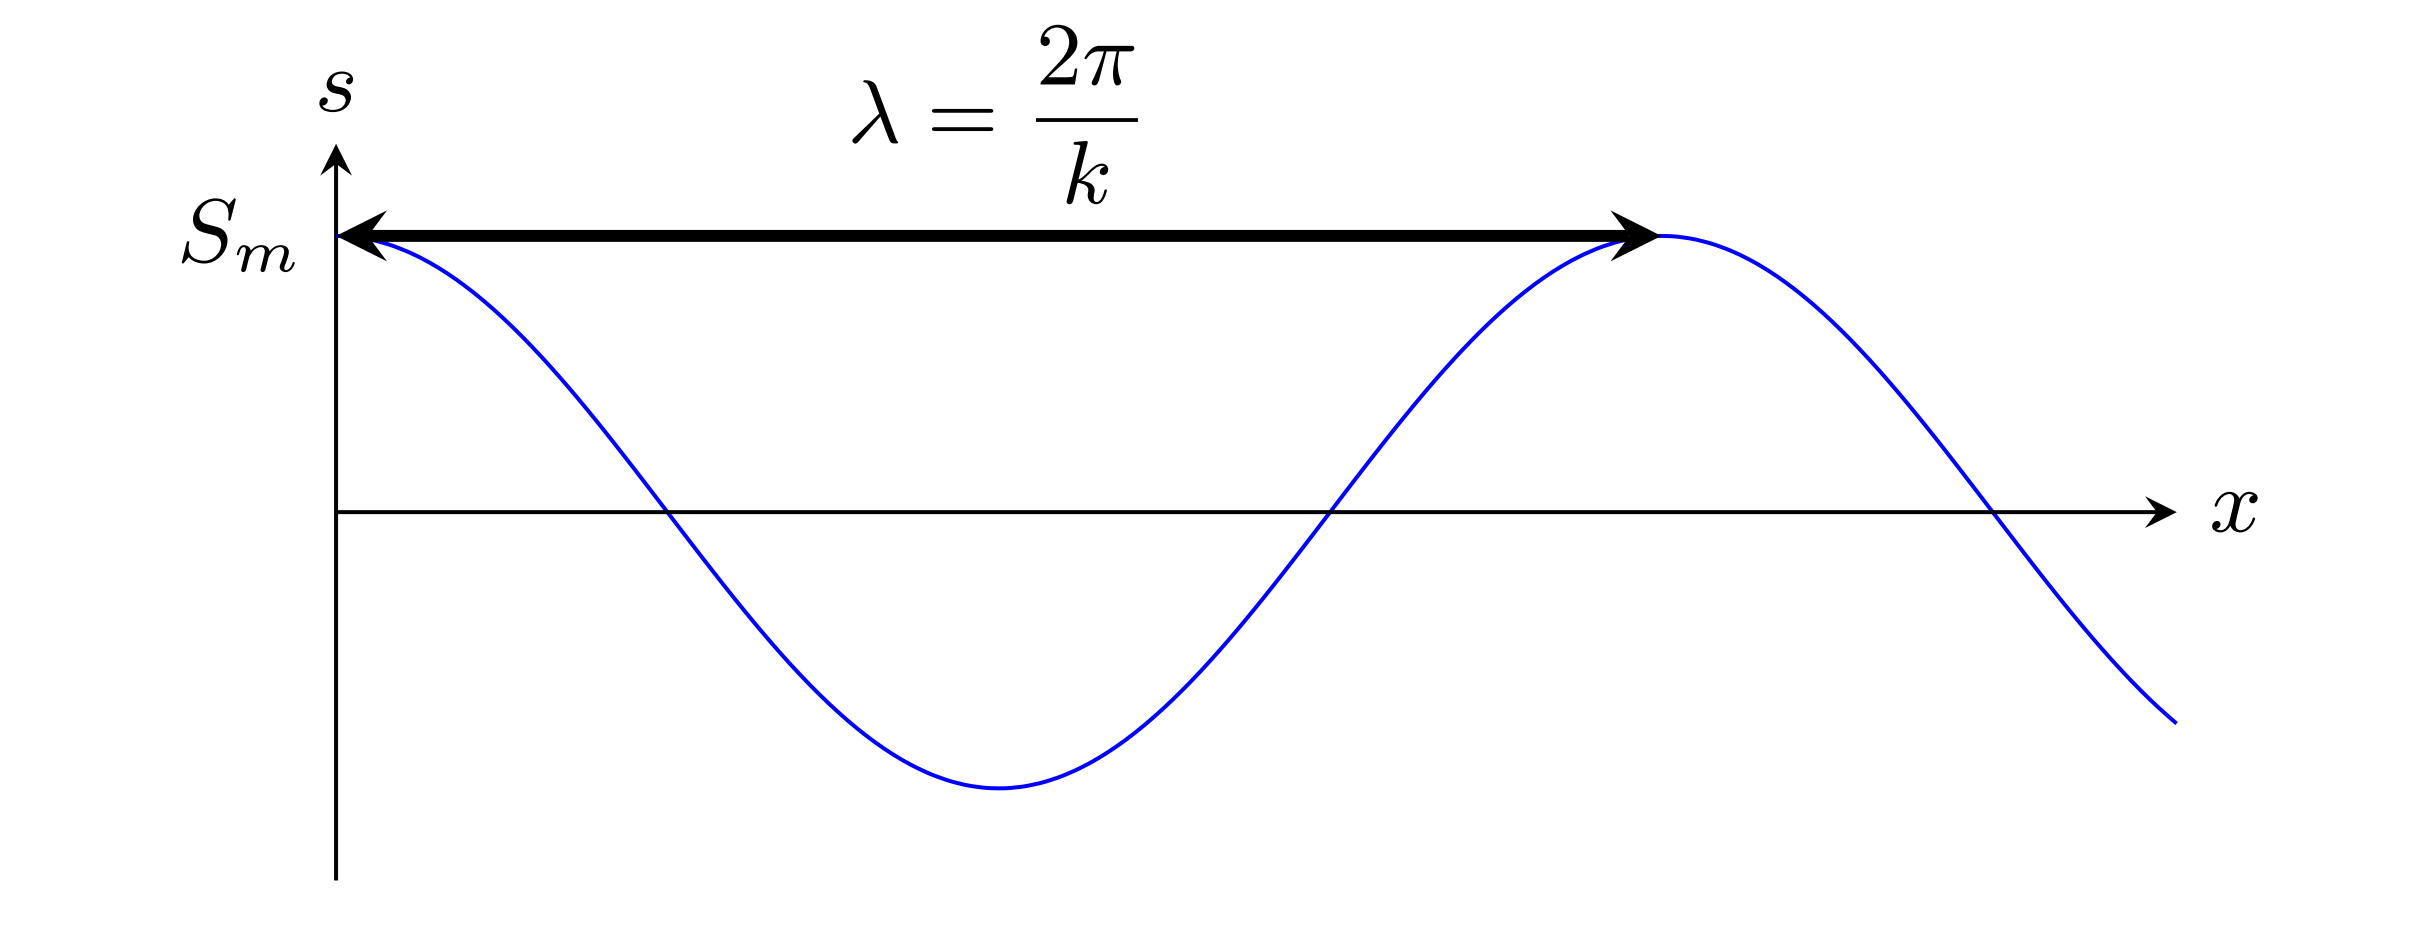
\includegraphics{png/evolution_spatiale.png}}
        \caption{Evolution spatiale du milieu à un instant donné.~\cite{propagation-onde}}
    \end{minipage}
\end{figure}

\paragraph{Calculs d'incertitudes}
La propagation d'incertitude basée sur le cours IPH est calculé de la manière 
suivante :~\cite{gravier-laurent}\\[2ex]
Relation :
\begin{align}
    g &= f(a) \\
    \Delta g &= |\frac{\partial f}{\partial a}|\Delta a + |\frac{\partial f}{\partial b}|\Delta b + |\frac{\partial f}{\partial c}|\Delta c + \ldots
\end{align}
L'incertitude $\Delta g$ est arrondi à 1 chiffre significatif selon le cours 
IPH.\\[2ex]
a, b, c sont les grandeurs physiques mesurées de manière directe. \\[2ex]
$\Delta a, \Delta b, \Delta c$ sont les incertitudes absolues des grandeurs 
a,b,c.\\[2ex]
$|\frac{\partial f}{\partial a}|;|\frac{\partial f}{\partial b}|;|\frac{\partial f}{\partial c}|$
sont les dérivées partielles de B par rapport à a, b, c.\\
\begin{align}
    \shortintertext{ Dans notre cas, la première méthode de mesure 
    nous donne une incertitude:}\notag\\
    \Delta c &= c \left( \frac{\Delta x}{x} + \frac{\Delta t}{t} \right) \\[2ex]
    \shortintertext{ $\Delta x$ $\pm$ 2 mm (valeur à ajuster)}
    \shortintertext{ $\Delta t$ $\pm$ 500 ms (valeur à ajuster)}\notag \\
    \shortintertext{ La deuxième méthode de mesure nous donne 
    une incertitude:}\notag  \\
    \Delta c &= c \left( \frac{\Delta \lambda}{\lambda} + \frac{\Delta f}{f} \right) \\[2ex] \notag 
    \shortintertext{ $\Delta \lambda$ $\pm$ 1 mm (valeur à ajuster)}
    \shortintertext{ $\Delta f$ $\pm$ 5 Hz (valeur à ajuster)} \notag
    \shortintertext{ L'équation (14) nous donne une incertitude:}
    \Delta c &= \frac{c}{2} \left( \frac{\Delta E}{E} + \frac{\Delta \rho}{\rho} \right)
    \shortintertext{ $\Delta E$ $\pm$ 10 $GPa$ (valeur à ajuster, sera prise d'internet)}
    \shortintertext{ $\Delta \rho$ $\pm$ 2 $\frac{kg}{m^3}$ (valeur à ajuster, sera prise d'internet)} \notag
    \shortintertext{ L'équation (15) nous donne une incertitude:}
    \Delta f &= f \left( \frac{\Delta c}{c} + \frac{\Delta d}{d} \right) \\[2ex]
    \shortintertext{ $\Delta c$ $\pm$ 2 $\frac{m}{s^2}$ (valeur à ajuster)}
    \shortintertext{ $\Delta d$ $\pm$ 1 mm (valeur à ajuster)}\notag \\
\end{align}

\newpage

\subsubsection{\large Protocole expérimental}
\paragraph{Présentation du montage}
\newpage
\section{Manipulation 2 "La vitesse de propagation du son dans des
barreaux solides d'au moins 3 matériaux différents."}
\subsection{Approches / Méthodes}
\subsubsection{\large Rappels Théoriques}
\paragraph{Introduction}
Quand une onde traverse un solide, 
sa célérité est tout sauf uniforme.
La célérité à laquelle une onde se déplace
dans un solide dépend intrinsèquement 
des caractéristiques de ce dernier.
Prenons l'exemple d'un violoncelle, 
le bois de l'instrument est choisi 
en raison de ses propriétés acoustiques 
particulières, notamment sa densité, son 
élasticité et sa configuration interne, 
favorisant ainsi une résonance optimale 
et une amplification efficace des vibrations 
des cordes.
Cette mélodie est rendue possible par la 
spécificité du bois du violoncelle, qui 
offre une célérité idéale pour la transmission 
des ondes sonores.
Maintenant, si nous prenons l'exemple d'une 
mine souterraine, où des explosifs sont 
utilisés pour creuser des tunnels.
Le son de l'explosion se propage à travers 
la roche, mais à une célérité bien plus 
élevée que dans le bois du violoncelle. 
Cette augmentation de vitesse est due à la 
nature plus rigide et dense de la roche, 
ce qui permet aux ondes sonores de se 
déplacer plus rapidement. Le but de cette 
expérimentation est de confirmer cela 
en mesurant la célérité du son dans différents 
matériaux.
\subsubsection{\large Protocole expérimental}
Le protocole expérimental est identique 
à celui de l'expérience précédente (Manipulation 1), 
à l'exception du fait que l'expérimentation 
est réalisée avec des barres de différents 
matériaux et de longueurs variables 
(100-200-400 mm).
\paragraph{Présentation du montage}
La configuration expérimentale employée 
pour mesurer la vitesse de propagation 
de l'onde est identique à l'expérience 
antérieure (Manipulation 1).

\newpage

\paragraph{Liste du matériel}
Le matériel utilisé est le même que 
celui de la première manipulation, 
avec l'ajout des barreaux suivants pour 
effectuer les mesures :
\begin{itemize}
    \item Tige matériaux et longueurs avec un diamètre de 10 mm:
    \subitem Aluminium 100, 200 mm.
    \subitem Laiton 100 mm.
    \subitem Cuivre 100 mm.
    \subitem Bois dur 200 mm.
    \subitem PVC 200 mm.
    \subitem Verre 200 mm.
    \subitem Verre acrylique 200 mm.
    \subitem Pom 200 mm.
    \subitem Nylon 200 mm.
\end{itemize}
\paragraph{Méthode de mesure}
La méthode de mesure et de calcul des 
incertitudes reste inchangée par rapport 
à l'expérience précédente (Manipulation 1). 
Afin de comparer les résultats en fonction 
du matériau, un graphique sera réalisé. 
Nous réaliserons les mesures de vitesses de 
propagation du son dans des barreaux solides 
d'au moins 3 matériaux différents.

\newpage

\subsection{\large Résultats / Analyse}
\subsubsection{\large Données brutes}
\paragraph{\large Aluminium 100 mm}
\paragraph{Tableau}
\paragraph{Graphe}
\paragraph{Observations}

\paragraph{\large Cylindre Acier inox 200 mm}
\paragraph{Tableau}
\paragraph{Graphe}
\paragraph{Observations}

\paragraph{\large Cylindre Acier inox 400 mm}
\paragraph{Tableau}
\paragraph{Graphe}
\paragraph{Observations}

\newpage

\subsubsection{\large Données réduites}
\paragraph{\large Cylindre Acier inox 100 mm}
\paragraph{Calculs}
\paragraph{Incertitudes}

\paragraph{\large Cylindre Acier inox 200 mm}
\paragraph{Calculs}
\paragraph{Incertitudes}

\paragraph{\large Cylindre Acier inox 400 mm}
\paragraph{Calculs}
\paragraph{Incertitudes}

\newpage

\subsubsection{\large Tableau récapitulatif}
\paragraph{Valeurs}
\paragraph{Incertitudes relatives}
\paragraph{Ecart relatif}

\subsubsection{\large Discussion quantitative}
\paragraph{Incertitude > écart}
validation
\paragraph{Incertitude < écart}
invalidation
discussion critique des méthodes
\newpage
\section{Manipulation 3 "Déterminer expérimentalement le module de Young d'au moins 3 matériaux."}
\subsection{Approches / Méthodes}
\subsubsection{\large Rappels Théoriques}
\paragraph{Introduction}
Au travers de cette manipulation, nous allons déterminer expérimentalement le module de Young de 
différents matériaux grâce à la mise en résonance de barreaux en utilisant la même méthode et montage
pour les mesures que dans les expérimentations précédentes. Grâce à la vitesse de propagation du son 
évaluée dans l'expérimentation précédente et la masse volumique des matériaux mesurée grâce à la 
méthode de la double pesée d'Archimède, nous allons déterminer le module de Young des matériaux.\\
Le module de Young ou module d'élasticité (longitudinal) est une constante intrinsèque
à chaque matériel qui relie la contrainte de traction ou de compression $[GPa]$ et la déformation 
$[-]$ élastique d'un matériel isotrope. Son symbole est E et son unité $[GPa]$. Ce module est une bonne
 approximation tant que la contrainte ne dépasse pas la limite élastique $Re$ du matériel. 
 ~\cite{wiki-mod-young}\\
La mesure de la densité $\rho$ par la méthode d'Archimède consiste à peser notre échantillon à vide
puis de le peser à nouveau immerger dans un liquide à la densité connue (dans notre cas de l'eau).\\
Afin de réaliser la mesure sur une balance de laboratoire, nous pesons directement la différence de
masse de liquide une fois l'échantillon immergé et stable. Cela permet également de réduire la 
propagation d'incertitude de la mesure en évitant de réaliser un delta de masse dispensable. \\
\begin{figure}[h]
    \centering
    \adjustbox{max width=\textwidth}{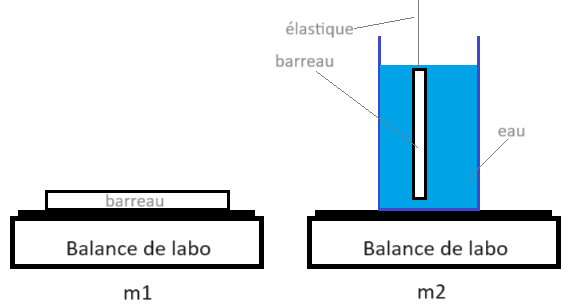
\includegraphics{doublePesee.png}}
    \caption{Double pesée}
\end{figure}\\
Il suffit ensuite d'appliquer la formule (23)
\newpage

\paragraph{Equations physiques}
\begin{align}
    \intertext{Masse volumique par la méthode de la double pesée : }
    \rho &= \rho_{l} \frac{m_{1} }{m_{2}}\\
    \shortintertext{ $\rho_{l} : $ masse volumique du liquide $[\frac{kg}{m^3}]$}
    \shortintertext{ $m_{1} : $ masse $[kg]$ }
    \shortintertext{ $m_{2} : $ masse immergée $[kg]$ } \notag
\end{align}
\begin{align}
    \intertext{Equation de d'Alembert sur l'axe Ox:}
    \frac{\partial^2 \xi}{\partial x^2} &= \frac{1}{c^2} \frac{\partial^2 \xi}{\partial t^2}\\
    \shortintertext{ $\xi : $ Gandeur physique portant l'onde $[\frac{[\xi]}{m^2}]$}
    \shortintertext{ $c : $ vitesse de propagation de l'onde $[\frac{m}{s}]$ }\notag
\end{align}
Ondes longitudinales dans un barreau solide ~\cite{Polycop-Ondes} :
\begin{figure}[h]
    \centering
    \adjustbox{max width=\textwidth}{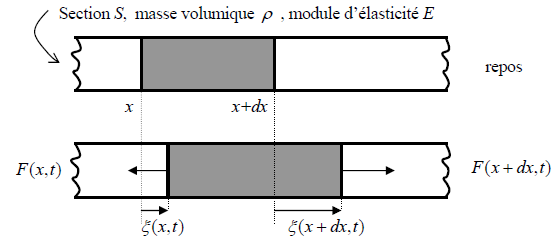
\includegraphics{OndesLongBarreauSol.png}}
    \caption{Barreau.~\cite{Polycop-Ondes}}
\end{figure}
\begin{align}
    \sigma(x,t)=\frac{F(x,t)}{S} &= E \frac{allongement}{longueur au repos} \notag \\
    &= E \frac{\xi(x+dx,t)-\xi(x,t)}{dx}\\
    \intertext{On peut en déduire l'équation de l'onde dans un barreau solide}
    \frac{\partial^2 \xi}{\partial x^2} &= \frac{\rho}{E} \frac{\partial^2 \xi}{\partial t^2}\\
    \shortintertext{ $\rho : $ masse volumique $[\frac{kg}{m^3}]$}
    \shortintertext{ $E : $ module d'élasticité du solide $[GPa]$}
    \intertext{Equation comparant l'équation de l'onde et celle de d'Alembert on obtient la propagation
     des ondes sinusoïdales dans les milieux solides (Equation 14) :}
    c &= \sqrt{\frac{E}{\rho}} \notag \\
    \implies E &= c^2 \rho 
    \shortintertext{ $c : $ vitesse de propagation de l'onde $[\frac{m}{s}]$}\notag
\end{align}
%\paragraph{Liste des paramètres}
%\begin{itemize}
 %   \item $\rho : $ masse volumique du matériel $[\frac{kg}{m^3}]$
  %  \subitem $m_{1} : $masse $[kg]$
   % \subitem $m_{2} : $masse immergée $[kg]$
    %\subitem $\rho_{l} : $masse volumique du liquide $[\frac{kg}{m^3}]$
%    \item $E : $module le Young du matériel $[Pa]$
 %   \item $v : $vitesse de propagation de l'onde $[\frac{m}{s}]$
%\end{itemize}
\paragraph{Calculs d'incertitudes}
La propagation d'incertitude basée sur le cours IPH est calculé de la manière 
suivante:~\cite{gravier-laurent}\\[2ex]
\begin{align}
    \intertext{Masse volumique : }
    \frac{\Delta \rho}{\rho} &= \frac{\Delta \rho_{l}}{\rho_{l}} + \frac{\Delta m_{1}}{m_{1}} + \frac{\Delta m_{2}}{m_{2}}\\
    \intertext{Module de Young : }
    \frac{\Delta E}{E} &= 2 \frac{\Delta c}{c} + \frac{\Delta \rho}{\rho}
\end{align}
\subsubsection{\large Protocole expérimental}
\begin{enumerate}
    \item Mesure de la masse volumique d'au moins 3 matériaux. 
    \subitem Suivant la méthode de la double pesée d'Archimède exprimée plus haut (équation 18). 
    \item Mesure de la longueur des barreaux au pied à coulisse
    \item Mise en résonance des différents barreaux sur notre montage expérimental pour en déduire la 
    vitesse de propagation du son dans le matériel
    \item Calcul avec leurs incertitudes des modules de Young des différents matériaux
\end{enumerate}

\paragraph{Présentation du montage}
Le montage utilisé pour la mesure de la vitesse de déplacement du son est exactement le 
même que dans les expérimentations précédentes.\\
Pour la mesure de la masse volumique, la méthode de la double pesée d'Archimède est utilisée. Le 
schéma est dans les rappels théoriques (Figure 5). %%%%% modifier numero 
Un élastique est utilisé pour accrocher le barreau à mesurer et le support de laboratoire. Il a l'avantage
de directement adhérer à la surface du barreau ce qui évite de devoir percer notre échantillon et 
fausser la mesure de la célérité. Son volume immergé et sa masse sont faibles et ne fausseront pas 
significativement nos mesures. Pour les matériaux dont la densité est plus faible que celle de l'eau, 
ils seront immergés à l'aide d'une fine pointe. De la même manière que pour l'élastique, les faibles
masse et volume de l'outil ne fausseront pas significativement nos résultats. 
\paragraph{Liste du matériel}
Mesures de la vitesse de propagation du son :\\
Le matériel utilisé est le même qu'à la manipulation précédente.\\
Mesure de la masse volumique :
\begin{itemize}
    \item Balance de laboratoire
    \item Long récipiant pour l'eau
    \item Supports de laboratoire
    \item Elastique
    \item Pointe fine
\end{itemize}
\paragraph{Méthode de mesure}
La méthode de mesure pour calculer la vitesse de propagation de l'onde $c$ est la même que pour 
l'expérimentation précédente.\\
Pour les masses, mesurées grâce à la balance de laboratoire, et les longueurs, mesurée au pied à 
coulisse les incertitudes sont calculées en fonction du nombre de chiffres significatif affiché sur 
l'appareille de mesure. \\
La masse volumique, calculé avec la méthode de la double pesée d'Archimède, l'incertitude est 
calculée suivant l'équation 29. L'incertitude relative de la masse volumique de l'eau sera de 0.5 pourcent
pour une valeur $\rho_{eau}=998[\frac{kg}{m^3}]$, car elle varie selon les conditions de température 
et de pression. Nous réaliserons les mesures de vitesses de 
propagation du son dans le but de calculer les modules de Young dans des
barreaux solides 
d'au moins 3 matériaux différents.

\newpage

\subsection{\large Résultats / Analyse}
\subsubsection{\large Données brutes}
\paragraph{\large Cylindre Aluminium 100 mm}
\paragraph{Tableau}
\paragraph{Graphe}
\paragraph{Observations}

\paragraph{\large Cylindre Acier inox 200 mm}
\paragraph{Tableau}
\paragraph{Graphe}
\paragraph{Observations}

\paragraph{\large Cylindre Acier inox 400 mm}
\paragraph{Tableau}
\paragraph{Graphe}
\paragraph{Observations}

\newpage

\subsubsection{\large Données réduites}
\paragraph{\large Cylindre Acier inox 100 mm}
\paragraph{Calculs}
\paragraph{Incertitudes}

\paragraph{\large Cylindre Acier inox 200 mm}
\paragraph{Calculs}
\paragraph{Incertitudes}

\paragraph{\large Cylindre Acier inox 400 mm}
\paragraph{Calculs}
\paragraph{Incertitudes}

\newpage

\subsubsection{\large Tableau récapitulatif}
\paragraph{Valeurs}
\paragraph{Incertitudes relatives}
\paragraph{Ecart relatif}

\subsubsection{\large Discussion quantitative}
\paragraph{Incertitude > écart}
validation
\paragraph{Incertitude < écart}
invalidation
discussion critique des méthodes
\newpage
\section{Manipulation 4 "Déterminer expérimentalement l'évolution du module
de Young en fonction de la longueur des barreaux pour au moins 
un matériau."}
\subsection{Approches / Méthodes}
\subsubsection{\large Rappels Théoriques}
\paragraph{Introduction}
Le Module de Young, la vitesse de propagation du son dans un solide et la densité étant des 
caractéristiques intrinsèques aux matériaux, si on varie la longueur de notre barreau, le module de 
Young devrait rester constant. Le but de cette expérimentation est de confirmer ce postulat en 
mesurant le module de Young de trois barreaux de longueurs différentes et de mêmes
matériaux et comparer les valeurs trouvées.
%\subsubsection{Les Rappels Théoriques}

%\paragraph{Liste des paramètres}
%\begin{itemize}
    %\item $\rho:$ masse volumique du matériel $[\frac{kg}{m^3}]$
    %subitem $m_{1}:$ masse $[kg]$
    %\subitem $m_{2}:$ masse immergée $[kg]$
    %\subitem $\rho_{l}:$ masse volumique du liquide $[\frac{kg}{m^3}]$
    %\item $E:$ module le Young du matériel $[Pa]$
    %\item $v:$ vitesse de propagation de l'onde $[\frac{m}{s}]$
%\end{itemize}
\subsubsection{\large Protocole expérimental}
Le protocole est le même que pour la manipulation précédente, à la nuance près que
l'essai se fait sur trois barreaux de même matériel et de longueur variable(100-200-400 mm).
Le matériel sera de l'acier inox, parce que c'est le seul dont nous disposons en 3 exemplaires de tailles 
différentes.

\paragraph{Présentation du montage}
Les montages utilisés pour la mesure de la vitesse de propagation du son et celui pour la masse volumique 
sont exactement les mêmes que dans les expérimentations précédentes. 

\paragraph{Liste du matériel}
Le matériel utilisé est le même qu'à la manipulation 4, à l'exception près des barreaux.
\begin{itemize}   
    \item Tige matériaux et longueurs avec un diamètre de 10 mm :
    \subitem Acier inox 100 mm
    \subitem Acier inox 200 mm
    \subitem Acier inox 400 mm
\end{itemize}
\paragraph{Méthode de mesure}
La méthode de mesure et celle de calcul des incertitudes sont exactement les mêmes que dans 
l'expérimentation précédente. Affin de comparer les résultats en fonction de la longueur du barreau, 
un graphique à moustaches sera effectué.

\newpage

\subsection{\large Résultats / Analyse}
\subsubsection{\large Données brutes}
\paragraph{\large Cylindre Aluminium 100 mm}
\paragraph{Tableau}
\paragraph{Graphe}
\paragraph{Observations}

\paragraph{\large Cylindre Acier inox 200 mm}
\paragraph{Tableau}
\paragraph{Graphe}
\paragraph{Observations}

\paragraph{\large Cylindre Acier inox 400 mm}
\paragraph{Tableau}
\paragraph{Graphe}
\paragraph{Observations}

\newpage

\subsubsection{\large Données réduites}
\paragraph{\large Cylindre Acier inox 100 mm}
\paragraph{Calculs}
\paragraph{Incertitudes}

\paragraph{\large Cylindre Acier inox 200 mm}
\paragraph{Calculs}
\paragraph{Incertitudes}

\paragraph{\large Cylindre Acier inox 400 mm}
\paragraph{Calculs}
\paragraph{Incertitudes}

\newpage

\subsubsection{\large Tableau récapitulatif}
\paragraph{Valeurs}
\paragraph{Incertitudes relatives}
\paragraph{Ecart relatif}

\subsubsection{\large Discussion quantitative}
\paragraph{Incertitude > écart}
validation
\paragraph{Incertitude < écart}
invalidation
discussion critique des méthodes
\newpage
\section{Manipulation 5 "Déterminer expérimentalement l'évolution du
module de Young en fonction de la température pour au moins un
matériau."}
\subsection{Approches / Méthodes}
\subsubsection{\large Rappels Théoriques}
\paragraph{Introduction}
    Après avoir mesuré la vitesse du son dans différents matériaux et
    calculé leur module de Young, nous nous intéressons maintenant à
    l'impact de la température sur ces mesures.
\paragraph{Equations physiques}
    Nous cherchons à exprimer le module de Young du matériau en fonction
    de la température à laquelle se trouve l'objet. Ceci dans le but
    d'évaluer l'influence de la température sur l'élasticité du matériau.
    ~\cite{Polycop-Ondes}
\begin{align}
    \intertext{
    Pour faire ceci nous allons utiliser la formule de la célérité du son
    utilisée l'équation 14}
    c &= \sqrt[]{\frac{E}{\rho}} => E = \rho c^2
    \intertext{Utilisons la formule de la dilatation volumique et les
    définitions de la masse volumique, du $\Delta \theta$ et du volume
    d'un cylindre :}
    V &= V_0(1+3\alpha \Delta \theta); V_0 = L_0 \frac{D_0^2\pi}{4};
    \rho = \frac{m}{V};\Delta \theta=\theta_f-\theta_i
    \intertext{Finalement on obtient :}
    E(\theta_f) &= \frac{4mc^2}{L_0D_0^2\pi\left(1+3\alpha(\theta_f-
    \theta_i)\right)}
\end{align}

Dans cette formule on a besoin de 5 paramètres fixes dépendants de notre
objet, soit la longueur initiale $L_0$ [m], le diamètre initial de notre
barre $D_0$ [m], sa masse $m$ [kg], le coefficient de dilatation linéique
du matériau $\alpha$ [1/°C] et la température à laquelle ont été mesurées
les dimensions initiales $\theta_i$ [°C].\\

Deux autres paramètres sont interdépendants : la température de l'objet
$\theta_f$ et la célérité du son mesurée $c$ [m/s] au moment de la
mesure.\\

Le résultat sera le module d'élasticité $E$ [GPa] du matériau à la
température $\theta_f$.\\

Pour les mesures de températures, nous avons décider d'utiliser les °C et
non les °K. En effet, l'unité d'un delta de température n'a pas
d'importance (Kelvin ou Celsius).
\paragraph{Calculs d'incertitudes}
    Selon la loi de propagations des incertitudes, nous pouvons en déduire
    l'erreur absolue sur le module de Young~\cite{gravier-laurent} :
    \begin{align}
    dE &= E \left(\frac{dm}{m}+2\frac{dc}{c}+\frac{\frac{dL_0}{L_0}+
    2\frac{dD_0}{D_0}+\left(\frac{dL_0}{L_0}+2\frac{dD_0}{D_0}+\frac{d
    \alpha}{\alpha}+\frac{d\theta_f+d\theta_i}{\theta_f-\theta_i}\right)
    \alpha(\theta_f-\theta_i)}{1+3\alpha (\theta_f-\theta_i)}\right)
    \end{align}
\subsubsection{\large Protocole expérimental}
    Cette expérience est un complément aux expériences précédentes. L'objet est
    chauffé uniformément en étant plongé dans un récipient d'eau
    chauffée avec une plaque chauffante. Lorsque celui-ci aura atteint la
    température voulue, nous le sortirons de l'eau. À partir de ce
    moment-là nous effectuerons des mesures régulières de la température
    au fur-et-à-mesure que celle-ci descend et de la célérité du son qui
    le traverse. 
\paragraph{Montage}

\begin{figure}[h]
    \centering
    \adjustbox{max width=\textwidth}{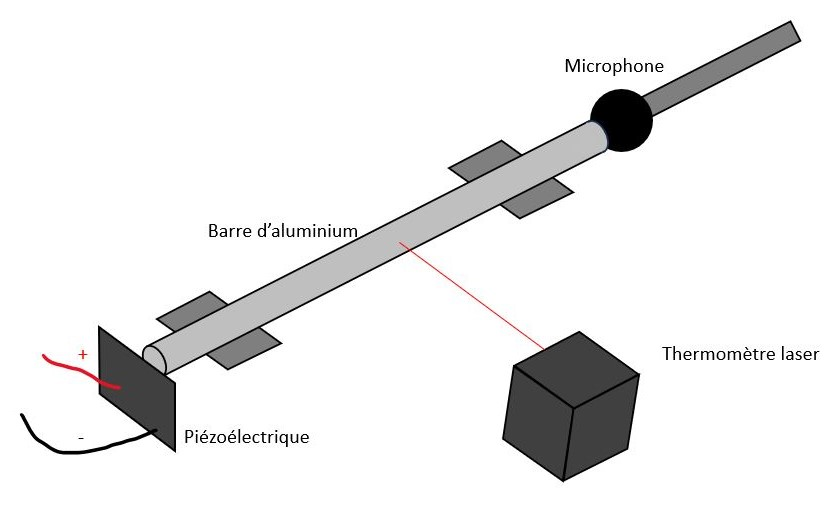
\includegraphics{montage_5.png}}
    \caption{Montage expérimental manipulation n°5}
\end{figure}
\newpage
\paragraph{Liste du matériel}
Le matériel utilisé est le même que 
celui de la première manipulation, 
avec l'ajout du matériel suivant pour 
effectuer les mesures :
\begin{itemize}
    \item Tige en aluminium, de longueur 100 mm et de diamètre 10 mm.\\
    \item Tige en acier inox, de longueur 100 mm et de diamètre 10 mm.\\
    \item Plaque chauffante\\
    \item Récipient chauffable\\
    \item Thermomètre laser\\
\end{itemize}

\paragraph{Méthode de mesure}
    Pour effectuer les mesures, il sera nécessaire d'avoir le moins
    de contact possible avec le matériau pour garder une température
    homogène. Pour faire ceci, nous allons utiliser un thermomètre laser.\\
    Faire des mesures sur un objet à une température homogène fixe
    ($\neq$ température de la salle) n'est pas facile, parce que celui-ci
    va vouloir tendre vers la température ambiante. Nous allons donc
    effectuer une série de mesures de température et de la célérité des
    vibrations d'une température proche de 100°C à une température
    approchant 20°C (idéalement entre 20 et 30 mesures). Ces mesures seront
    entrées dans un tableau Excel qui tracera la courbe de variation du
    module de Young.


\newpage

\subsection{\large Résultats / Analyse}
\subsubsection{\large Données brutes}
\paragraph{\large Cylindre Aluminium 100 mm}
\paragraph{Tableau}
\paragraph{Graphe}
\paragraph{Observations}

\paragraph{\large Cylindre Acier inox 100 mm}
\paragraph{Tableau}
\paragraph{Graphe}
\paragraph{Observations}

\newpage

\subsubsection{\large Données réduites}
\paragraph{\large Cylindre Aluminium 100 mm}
\paragraph{Calculs}
\paragraph{Incertitudes}
\paragraph{Régression Linéaire}

\paragraph{\large Cylindre Acier inox 100 mm}
\paragraph{Calculs}
\paragraph{Incertitudes}
\paragraph{Régression Linéaire}
\newpage

\subsubsection{\large Tableau récapitulatif}
\paragraph{Valeurs}
\paragraph{Incertitudes relatives}
\paragraph{Ecart relatif}

\subsubsection{\large Discussion quantitative}
\paragraph{Incertitude > écart}
validation
\paragraph{Incertitude < écart}
invalidation
discussion critique des méthodes
\newpage

%\section{Références bibliographiques}
%\printbibliography[heading=none]



\begin{figure}
    \centering
    
\includegraphics[width=0.6\textwidth]{HEIG_1.png}
    \caption{Légende de la première figure}
  \end{figure}

\begin{table}[h] % [h] indique que le tableau doit être placé ici (ou utilisez [ht] pour plus de contrôle)
    \centering % Centre le tableau dans la page
    \caption{Titre de votre tableau} % Ajoutez une légende au tableau
    \begin{tabular}{|c|c|c|} % Définit le format des colonnes (ici, 3 colonnes centrées avec des barres verticales)
        \hline % Ligne horizontale en haut du tableau
        Colonne 1 & Colonne 2d & Colonne 3 \\ % Contenu de la première ligne du tableau
        \hline % Ligne horizontale
        Valeur 1 & Valeur 2 & Valeur 3 \\ % Contenu de la deuxième ligne
        Valeur 4 & Valeur 5 & Valeur 6 \\ % Contenu de la troisième ligne
        \hline % Ligne horizontale en bas du tableau
    \end{tabular}
\end{table}
\newpage

\raggedright % Ajoutez cette commande pour éviter les erreurs de dépassement des marges
\printbibliography[heading=bibintoc, title={Bibliographie}] % Bibliographie
\end{document}
